% Chapter 7
\section{Inference at Scale: False Discovery Rate Control}\label{sec:fdr}

Section~\ref{sec:debiased} upgraded a single coefficient $\beta_j$ from a point estimate to a $p$-value. But the applied scientist never tests just one hypothesis: a single genomic screen tests $d \approx 2\times 10^4$ genes at once, a marketing review inspects hundreds of segmented metrics, an epidemiological analysis regresses on dozens of exposures. \textbf{Chapter 6 answered ``is \emph{this} coefficient significant?''; this chapter answers ``of this entire page of conclusions, how many are real''} — the last mile before regression output becomes a \textbf{credible scientific assertion}, and the closing of the loop from sparse estimation to FDR control.

\subsection{Where the Problem Starts: Multiple Testing and the Credibility of Discoveries}\label{sec:fdr-problem}

Suppose we have $m$ hypotheses $H_1, \dots, H_m$ (e.g.\ $H_j: \beta_j = 0$) with $p$-values $p_1, \dots, p_m$, of which $m_0$ are true. Testing each $p$-value at level $\alpha$ individually, if all $m_0$ null hypotheses were true, the probability of at least one false rejection is as high as
\[
  1 - (1 - \alpha)^{m_0} \ \approx\ 1 - e^{-\alpha m_0}
  \qquad (\text{almost certain for large } m_0).
\]
With $m = 10^4$ and $\alpha = 0.05$ this is essentially $100\%$ ($1 - 0.95^{10^4} \approx 1 - e^{-513}$) — \textbf{``this page is entirely false discoveries'' is not an accident; it is the default outcome}.

The classical remedy is to control the \textbf{family-wise error rate} (FWER): $\mathrm{FWER} = \Prob( V \ge 1 )$, where $V$ is the number of false rejections. The Bonferroni method compresses each test's threshold to $\alpha/m$: FWER $\le \alpha$ indeed holds, but at the price of a threshold that \textbf{tightens linearly in $m$}. At $m = 10^4$ the threshold is $5\times 10^{-6}$: unless the effect is enormous, \emph{nothing can be rejected} — the errors are controlled, and so are the discoveries.

In 1995 Benjamini and Hochberg proposed a question better matched to ``screening'' scenarios\cite{benjamini1995}: promise not ``never make a single mistake'' but control the \textbf{false discovery rate}
\begin{equation}\label{eq:fdr-def}
  \mathrm{FDR} = \E\Big[ \frac{V}{\max(R, 1)} \Big],
  \qquad R = \text{total number of rejections}.
\end{equation}
$V/R$ is \textbf{the fraction of false discoveries among the rejected} (with the convention $0$ when $R = 0$). FDR allows false discoveries but requires them to be controlled \emph{in proportion} — the more discoveries, the more false ones tolerated; and when nothing can be rejected, no debt is owed. FWER and FDR relate in one line (Exercise~\ref{ex:bh-bonf}):
\[
  \mathrm{FDR} \le \mathrm{FWER},
\]
so Bonferroni, which controls FWER, necessarily controls FDR — just far too conservatively. The division of labor is therefore clear: \textbf{confirmatory} settings (one assertion going to court, onto a drug label) demand FWER; \textbf{exploratory} settings (screening candidate genes, shortlisting metrics) should use FDR.

\subsection[The Benjamini--Hochberg Procedure: Ranking, a Sloped Line, and the Last Crossing Point]{The Benjamini--Hochberg Procedure: Ranking, a Sloped Line, and the Last Crossing Point}\label{sec:bh}

The BH procedure is disarmingly simple. Sort the $p$-values $p_{(1)} \le \dots \le p_{(m)}$; given a target level $q \in (0, 1)$, define
\begin{equation}\label{eq:bh}
  \hat{k} = \max\Big\{ k :\ p_{(k)} \le \frac{q\, k}{m} \Big\},
  \qquad
  \text{reject } H_{(1)}, \dots, H_{(\hat{k})}
  \ \ \text{(if no such $\hat{k}$ exists, reject nothing).}
\end{equation}
Geometrically (Figure~\ref{fig:ch7-fdr}(a)): plot the sorted $p$-values as a staircase and find the \textbf{last crossing point} with the sloped line $qk/m$. Bonferroni is the horizontal line $q/m$ (a single point at $k=1$); BH relaxes the threshold \emph{linearly} in the rank $k$ — the $k$-th smallest $p$-value faces a hurdle $k$ times Bonferroni's.

\begin{theorem}[Benjamini--Hochberg, 1995]\label{thm:bh}
If the $p$-values are independent, or more generally satisfy a positive-regression-dependence condition (PRDS), then the BH procedure \eqref{eq:bh} satisfies
\[
  \mathrm{FDR} \le \frac{m_0}{m}\, q \ \le\ q .
\]
\end{theorem}
The full proof under independence is the guided induction of Exercise~\ref{ex:bh-proof}; here is the intuition. The false-discovery proportion is adjudicated by the \emph{slope} of the line: the relaxation rate of $qk/m$ is calibrated so that per $k$ rejections, at most $qk$ false ones are budgeted. False discoveries enter the rejection set by ``smuggling in as small $p$-values among the real signals''; and when real signals exist, $\hat{k} \gg 1$, so the threshold $q\hat{k}/m$ relaxes by orders of magnitude relative to $q/m$ — \textbf{the more discoveries, the looser each individual hurdle, but the total budget is locked at $q$}. This is the precise mechanism of ``tolerate a few false ones when there are many discoveries.''

\begin{figure}[htbp]
  \centering
  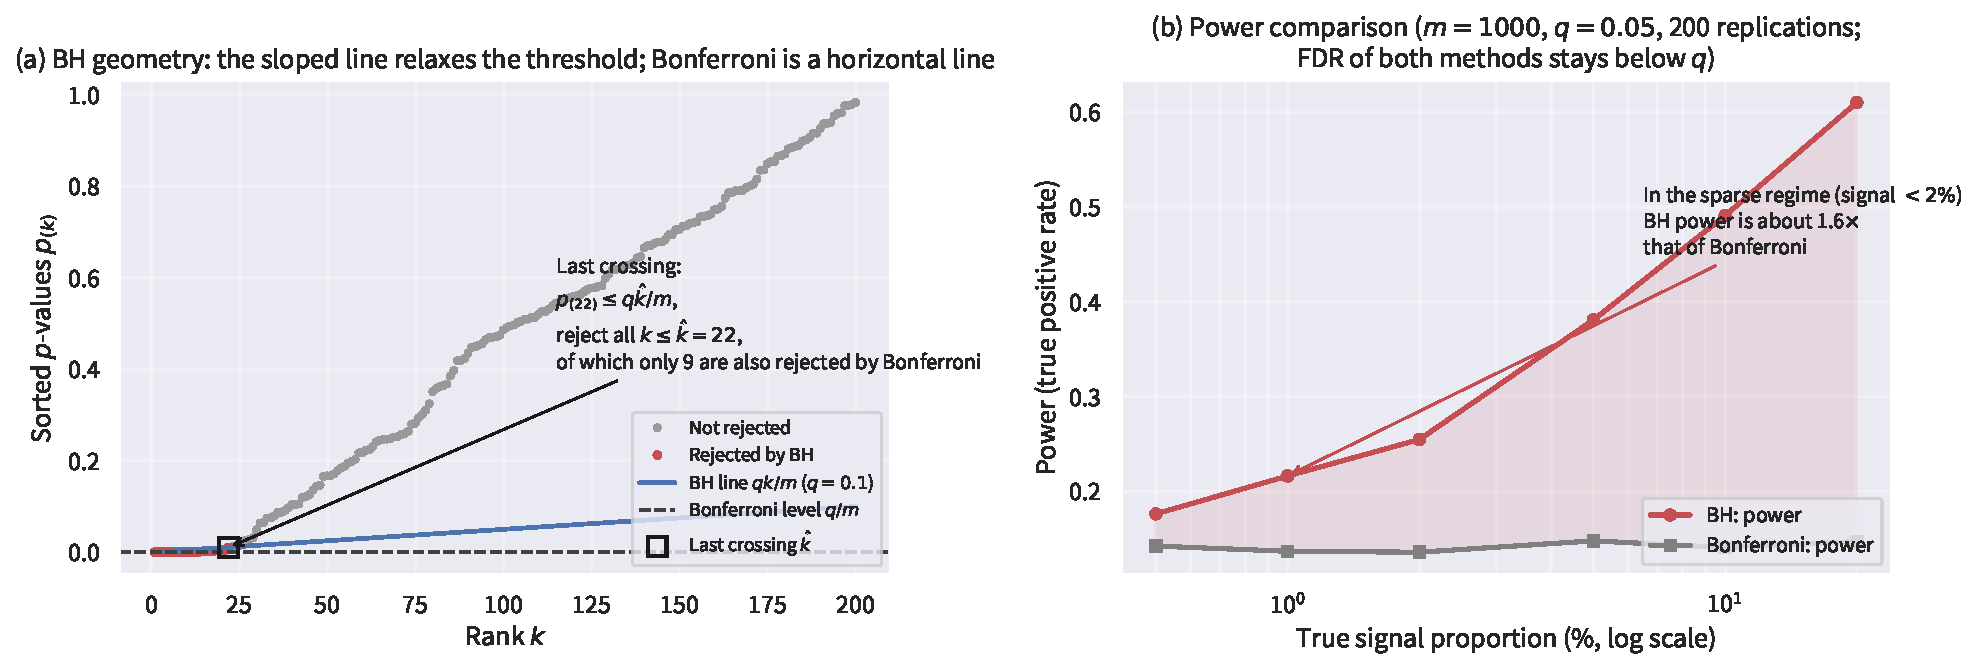
\includegraphics[width=\linewidth]{figures/ch7_fdr.pdf}
  \caption{(a) The geometry of BH (one simulation: $m=200$ independent tests, of which 30 signals with $z_j \sim \mathcal{N}(3.2, 1)$, $q=0.1$): the staircase of sorted $p$-values crosses the sloped line $qk/m$ for the last time at $\hat{k}=22$, and all $k\le 22$ are rejected; Bonferroni's horizontal line $q/m$ would reject only 9 of them. (b) A power simulation ($m=1000$, $q=0.05$, 200 replications): as the signal fraction varies from $0.5\%$ to $20\%$ ($z_j \sim \mathcal{N}(3,1)$), the power of BH rises from $0.18$ to $0.61$ while Bonferroni's stays pinned near $0.14$; at a $1\%$ signal fraction BH's power is about $1.6\times$ Bonferroni's. Both procedures keep the measured FDR at or below $q$ (BH between $0.038$ and $0.054$, Bonferroni between $0.0008$ and $0.045$) — \textbf{the power bought by the sloped line costs not a cent of error rate}.}
  \label{fig:ch7-fdr}
\end{figure}

\subsection{Closing the Loop: BH Is an Adaptive Sparse Estimator}\label{sec:fdr-sparsity}

Now back to this book's main line — sparsity. Transform one-sided $p$-values into $z$-scores $z_j = \Phi^{-1}(1 - p_j)$; the BH procedure is equivalent to finding a \textbf{data-driven cutoff} on the ordered $z$-scores: reject $z_{(j)} \ge \hat{t}$. This cutoff is not the pre-specified $\sqrt{2 \log m}$; it ``grows'' out of the data itself — and where it lands depends on how sparse the signals are.

Abramovich, Benjamini, Donoho, and Johnstone (2006) turned this observation into a theorem\cite{abramovich2006}. Consider the sparse normal means model
\[
  z_j = \theta_j + \varepsilon_j, \qquad \varepsilon_j \sim \mathcal{N}(0, 1),
  \qquad \#\{ j : \theta_j \neq 0 \} \le s \ll m,
\]
and use the BH cutoff at an appropriate level $q$ as a \emph{threshold estimator} $\hat\theta_j = z_j \cdot \ind{ z_j \ge \hat{t} }$ (hard thresholding). The core result: \textbf{without knowing the sparsity $s$, this FDR-controlled rule automatically achieves the same minimax risk rate as the oracle threshold that \emph{knows} $s$} — squared risk on the order of $2 s \log(m/s)$ (up to constant factors), rather than the $2 s \log m$ delivered by the non-adaptive threshold $\sqrt{2 \log m}$. When $s \ll m$, $\log(m/s) \ll \log m$, and the gap is substantial.

Placed side by side with Section~\ref{sec:ggm-estimate}, the same face appears twice:
\begin{center}
\resizebox{\textwidth}{!}{%
\begin{tabular}{@{}lll@{}}
\toprule
 & Sparse estimation (Chapter 6) & FDR testing (this section) \\
\midrule
Object & regression coefficients $\bbeta$ or means $\bm{\theta}$ & a family of hypotheses $H_1, \dots, H_m$ \\
Mechanism & $\ell_1$ penalty / soft thresholding & sorted $p$-values / BH threshold \\
Source of adaptivity & penalty parameter $\lambda$ via cross-validation or BIC & cutoff located automatically by the crossing point \\
Role of sparsity & makes estimation possible when $d \gg n$ & lets the BH cutoff drop automatically to the signal layer \\
\bottomrule
\end{tabular}}
\end{center}
\textbf{Controlling the false discovery rate is not a patch on top of estimation; it is the dual formulation of the sparsity assumption on the testing side}: ``most coefficients are zero'' both enables the lasso to estimate and enables BH to adaptively find its threshold. Donoho's name appears once in Chapter 6 (the compressed-sensing tradition) and once in this section — no coincidence: it is the same logic chain ``sparsity $\Rightarrow$ thresholding $\Rightarrow$ optimality,'' seen from its two ends.

\subsection[Back to Regression I: Debiased Lasso $p$-Values Through BH]{Back to Regression I: Debiased Lasso $p$-Values Through BH Control the FDR of Coefficients}\label{sec:fdr-regression}

The pipeline is already in place: Section~\ref{sec:debiased} gives the asymptotic normality of $\sqrt{n}(\widetilde{\beta}_j - \beta_j)$ in \eqref{eq:asym-norm}, hence an asymptotic $p$-value $p_j$ for every $H_{0j}: \beta_j = 0$. Feed the $d$ $p$-values to BH \eqref{eq:bh}; by Theorem~\ref{thm:bh} — provided the $p$-values are approximately independent or positively correlated — \textbf{the false discovery rate of the rejected coefficient set is controlled at $q$}. Combined with the correspondence $\beta_j = 0 \Leftrightarrow y \perp x_j \mid \x_{-j}$ of Section~\ref{sec:beta-theta}, this is the standard endpoint of conditional-independence structure screening in high-dimensional regression: lasso proposes candidate edges, the debiased lasso produces $p$-values, BH certifies credibility.

Following this book's custom, three honest caveats, disclosed one by one:
\begin{enumerate}[label=(\roman*)]
  \item \textbf{The $p$-values are asymptotic}. \eqref{eq:asym-norm} is a large-sample statement; in finite samples BH's control is approximate, and the larger $d$ is relative to $n$, the more the approximation leans on the sparsity conditions.
  \item \textbf{Correlation structure}. The debiased $p$-values are correlated through the design matrix. Extreme collinearity (the ill-conditioning of Section~\ref{sec:hd-break}) can break the PRDS condition, and the measured FDR can overshoot; under general dependence there is the more conservative Benjamini--Yekutieli correction\cite{benjamini2001} (replace $q$ by $q / \sum_{j=1}^m j^{-1} \approx q / \log m$), at a cost in power.
  \item \textbf{Consistency of screening and inference objects}. If lasso is used to pre-screen variables and tests are performed only on the survivors, standard BH theory no longer applies directly (the selection itself introduces extra randomness) — precisely the pitfall the method of the next section is designed to bypass.
\end{enumerate}

\subsection[Back to Regression II: Knockoffs]{Back to Regression II: Knockoffs — FDR Control Without $p$-Values}\label{sec:knockoffs}

Barber and Candès (2015) took a more radical route\cite{barber2015}: \textbf{instead of manufacturing $p$-values and correcting them afterward, construct ``mirror variables'' inside the design matrix and let symmetry itself bear the control}. For each column $\x_j \in \R^n$, construct a knockoff $\tilde{\x}_j$ such that \textbf{swapping any pair $(\x_j, \tilde{\x}_j)$ leaves the joint distribution of the augmented design $[\X\ \tilde{\X}]$ unchanged} (the exchangeability property). For Gaussian designs there is an explicit construction — and it requires second-order information about the correlations among the columns of $\X$, i.e.\ \textbf{we are back to the covariance/precision matrices of Section~\ref{sec:cov-prec}}: each knockoff is calibrated to its original so that the more strongly correlated a variable, the more convincing its mirror. (A remark on conventions: the original Barber--Candès \textbf{fixed-$X$} construction requires $n \ge 2d$; the second-order construction described here is the \textbf{model-X} Gaussian version, whose high-dimensional construction remains an active research direction.)

Next define an importance score $Z_j$ for each variable and $\tilde{Z}_j$ for its knockoff (e.g.\ the lasso-path order in which the variable enters the model), and combine them into the \textbf{signed statistic}
\[
  W_j = Z_j - \tilde{Z}_j ,
\]
whose sign records whether the original beats its mirror. The key observation: under $H_{0j}$ ($\x_j$ is independent of $\y$), the original and the knockoff are indistinguishable, and exchangeability gives
\begin{equation}\label{eq:knockoff-sym}
  W_j \ \overset{d}{=}\ -W_j
  \qquad (H_{0j}, \text{ conditional on everything else}),
\end{equation}
i.e.\ \emph{the $W_j$ of null variables are symmetric about $0$}, while true signals push $W_j$ toward large positive values. The count of \emph{negative} $W$'s therefore becomes a \textbf{symmetry-based estimate of the false discovery count}: ordering by $|W_j|$ from largest to smallest, the knockoff+ procedure takes the threshold
\begin{equation}\label{eq:knockoff}
  T = \min\Big\{ t > 0 :\ \frac{ 1 + \#\{ j : W_j \le -t \} }{ \#\{ j : W_j \ge t \} } \le q \Big\},
  \qquad
  \text{reject } \{ j : W_j \ge T \}.
\end{equation}
The ``$1+$'' in the numerator is an overdispersion correction for the randomness; and \eqref{eq:knockoff-sym} guarantees that each falsely rejected variable contributes a negative mirror with probability $1/2$ — the very fulcrum of the proof. The conclusion holds under \emph{any} model (no linearity, no asymptotics):
\[
  \mathrm{FDR} \le q .
\]

The two routes, side by side:
\begin{center}
\resizebox{\textwidth}{!}{%
\begin{tabular}{@{}lll@{}}
\toprule
 & BH $+$ debiased lasso (Section~\ref{sec:fdr-regression}) & Knockoffs (this section) \\
\midrule
Fulcrum of control & asymptotic normality of $p$-values & exchangeability symmetry of the design \\
Model assumptions & required (linearity $+$ sparsity $+$ asymptotics) & none (model-free) \\
Finite-sample guarantee & approximate (asymptotic) & \textbf{exact} (finite-sample) \\
Extra cost & nodewise estimation needed for debiasing & constructing knockoffs (fixed-$X$ construction needs $n \ge 2d$; model-X needs a known or estimable feature distribution) \\
\bottomrule
\end{tabular}}
\end{center}

At this point the ``credible scientific assertion'' toolkit is complete: the debiased lasso gives \textbf{single}-coefficient $p$-values (Section~\ref{sec:debiased}), BH gives FDR control for a \textbf{page} of $p$-values (earlier in this chapter), and knockoffs give model-free, finite-sample-exact FDR control for \textbf{variable selection} (this section). Candès and Donoho are honored in the preface because the modern credibility theory of regression happens to have been written by these two schools — one showing that \emph{sparsity makes estimation possible}, the other that \emph{symmetry makes inference credible}.

\begin{keybox}[Chapter takeaways]
\begin{itemize}
  \item Under multiple testing, Bonferroni controls FWER but its $\alpha/m$ threshold tightens linearly in $m$ and power collapses; FDR $= \E[V/\max(R,1)]$ allows ``tolerate a few false ones when there are many discoveries'' — the right currency for exploratory screening (Section~\ref{sec:fdr-problem});
  \item The BH procedure $=$ the last crossing point of sorted $p$-values with the sloped line $qk/m$; under independence (or PRDS), $\mathrm{FDR} \le q\, m_0/m \le q$ (Theorem~\ref{thm:bh});
  \item Closing the loop: the BH threshold is an adaptive sparse estimator of the $z$-scores, achieving oracle-level minimax rates without knowing the sparsity\cite{abramovich2006} — false discovery control and sparse estimation are one coin;
  \item The regression pipeline: debiased lasso emits $p$-values, BH controls FDR — but asymptotic approximation and collinearity are honestly disclosed weaknesses; knockoffs use the exchangeability symmetry of mirror variables to give model-free, finite-sample-exact FDR control\cite{barber2015}.
\end{itemize}
\end{keybox}

\begin{exercise}\label{ex:bh-hand}
$m = 5$, $q = 0.1$, and five (already sorted) $p$-values $0.001,\ 0.02,\ 0.04,\ 0.09,\ 0.3$. Execute BH step by step: write down the threshold $qk/m$ for each $k$, the decision, $\hat{k}$, and the final rejection set; then compare the rejection sets of BH, Bonferroni (threshold $q/m$), and naive per-test testing at level $q$.
\end{exercise}

\begin{exercise}\label{ex:bh-bonf}
(a) Prove $\mathrm{FDR} \le \mathrm{FWER}$, and conclude that any procedure controlling FWER (e.g.\ Bonferroni) automatically controls FDR; (b) prove that the Bonferroni rejection set at level $q$ is a subset of the BH rejection set at level $q$; (c) Let $m = 10^5$ independent tests include $200$ signals with $z_j \sim \mathcal{N}(5, 1)$ (two-sided $p$-values), $q = 0.05$. Estimate Bonferroni's per-test threshold and power, quantify how much looser the BH threshold is at $\hat{k} \approx 200$, and explain why BH's power then tends to $1$ while Bonferroni's falls well short.
\end{exercise}

\begin{exercise}[Proof sketch, harder]\label{ex:bh-proof}
Under \textbf{all $m$ hypotheses true} and \textbf{independent} $p$-values, prove $\Prob( \exists k : p_{(k)} \le qk/m ) \le q$ (under the complete null, $\mathrm{FDR}$ equals this probability, so the worst case of Theorem~\ref{thm:bh} holds). Complete the following skeleton: (i) induct on $m$, with $m = 1$ trivial; (ii) key step: condition on the largest order statistic $p_{(m)}$ and split into the cases $p_{(m)} \le q$ and $p_{(m)} = u > q$; use the fact that, given $p_{(m)} = u$, the remaining $m-1$ variables are $m-1$ independent $U(0, u)$ variables divided by $u$, rewrite the event as the same event for $m-1$ uniforms, and verify that the level parameter changes from $q$ to $q' = q(m-1)/(m u)$; (iii) combine the two cases.
\end{exercise}

\begin{exercise}\label{ex:knockoff}
(a) Use exchangeability to show carefully: under $H_{0j}$, globally swapping $\x_j$ with $\tilde{\x}_j$ leaves the joint distribution of the statistic vector $(W_1, \dots, W_m)$ invariant while flipping the sign of $W_j$ — hence \eqref{eq:knockoff-sym} (hint: under $H_{0j}$, $\y$ does not depend on $\x_j$, so the swap does not change the regression problem); (b) explain why $\#\{j : W_j \ge t\}$ in the denominator of \eqref{eq:knockoff} counts ``discoveries with $|W|$ above $t$,'' and why (up to the $1+$) $\#\{j : W_j \le -t\}$ is an \textbf{estimate of the false-discovery count} — and how symmetry turns this estimate into the fulcrum of an upper bound in expectation.
\end{exercise}
